\section{Overall Design}
\label{sec:design}

\begin{figure}[!t]
	\center
	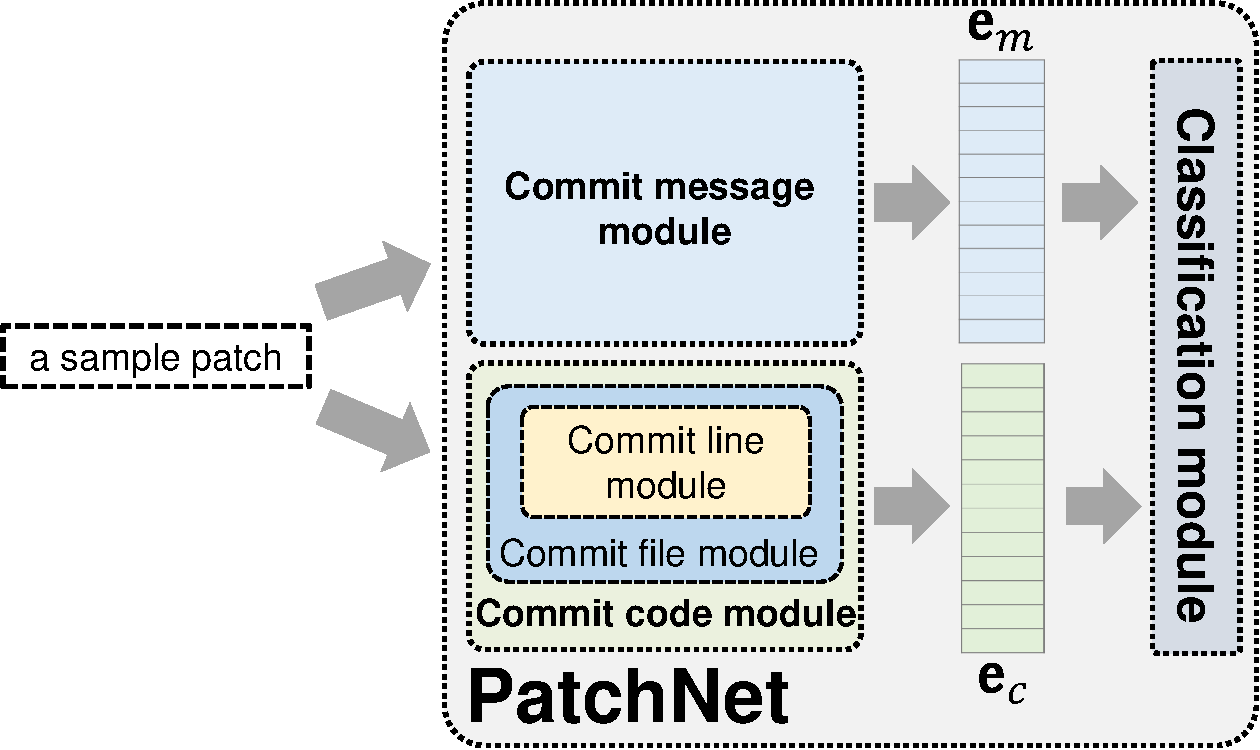
\includegraphics[scale=0.38]{figures/overall_patchnet.pdf}
	\caption{The proposed PatchNet framework. $\textbf{e}_m$ and $\textbf{e}_c$ are embedding vectors collected from the commit message module and commit code module respectively.}
	\label{fig:patchnet}
    \vspace{-0.4cm}
\end{figure}

Figure~\ref{fig:patchnet} shows an overall framework of our PatchNet. Our tool accepts as input a set of patches, which contain both commit messages and commit code. The output of PatchNet is a list of predicted scores reflecting how likely the given patches are bug fixing patches. Our framework includes three main modules: the \textit{commit message module}, the \textit{commit code module}, and the \textit{classification module}. The commit message module and the commit code module transform the commit message and the commit code into embedding vectors $\text{e}_m$ and $\text{e}_c$, respectively. The two vectors are then passed to the classification module, which aims to compute a prediction indicating the likelihood of a patch being bug fixing patch. 

\noindent \textbf{Commit message module:} This module takes a commit message as input and outputs an embedding vector that represents the most salient features of the message. The commit message module is the same as the one proposed by Kim~\cite{kim2014convolutional} for sentence classification. 